\documentclass[12pt, fleqn]{article}
\usepackage[serbian]{babel}


\usepackage{thesis}
\newcommand{\thesisName}{Hardverska implementacija Viola-Jones algoritma}

\author{Risto Pejašinović}
\date{}


\begin{document}
%% listing and figure numbering per section %%
\counterwithin{lstlisting}{section}
\counterwithin{figure}{section}
\counterwithin{equation}{section}
\counterwithin{table}{section}

\maketitle
\thispagestyle{empty}
\newpage

\tableofcontents
\newpage

\section{Viola-Jones algoritam}

\subsection{Uvod}

Namena algoritma je detekcija i lokalizacija objekata na slici. Osmišljen od
strane Paul Viola i Michael Jones 2001. godine \cite{Viola2001RapidOD}.

Dugo godina je zbog brze i pouzdane detekcije bio standardan način detekcije
lica na slici. I danas je prisutan u velikom broju mobilnih telefona i
digitalnih kamera, ali danas postaje polako zamenjen konvolucionim neuronskim
mrežama. \\

Pouzdanost i brzina su postignuti uvođenjem tri ključna doprinosa:
\begin{itemize}

\item \textbf{Integralna slika} omogućava brzo izračunavanje obeležja.
\item \textbf{AdaBoost} algoritam za učenje, odabiranjem obeležja povećava
  brzinu i pouzdanost detekcije.
\item \textbf{Kaskadni klasifikator} Realizovanjem algoritma u kaskadama
  omogućava brzo odbacivanje pozadine slike kako je mala verovatnoća da će se tu
  naći lice. \\
\end{itemize}


\subsection{Integralna slika}

Kao jedan od ključnih delova algoritma, integralna slika omogućava izračunavanje
površine svakog pravougana obeležja u konstantnom vremenu.

Intenzitet piksela u integralnoj slici na poziciji x,y je zbir svih piksela koji
se nalaze gore i levo od pozicije x,y.

\begin{equation}
  \Scale[1.4]{ii(x,y)=\sum\limits_{x'\leq x, y'\leq y} i(x',y')}
  \label{IntegralImage_eq1}
\end{equation}

Gde je ii(x,y) integralna slika, a i(x,y) originalna slika. \\

\begin{figure}[h]
  \centering
  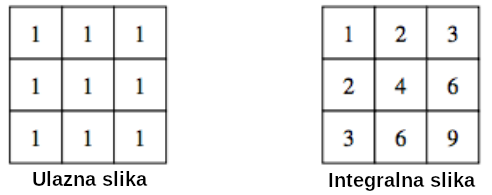
\includegraphics[width=8cm]{integral_image1}
  \caption{Primer integralne slike}
  \label{IntegralImage_img1}
\end{figure}

Piksele integralne slike je moguće računati u paraleli, ili
sekvencijalno. Izbor algoritma za računanje integralne slike značajno utiče na
performanse i potrebne hardverske resurse. \\
U paralelnoj implementaciji cena je
više pristupa memoriji i više potrebnih sabirača, dok je kod sekvencijalne
implementacije manja brzina. \\

Osobina koja integralnu sliku čini pogodnu za korišćenje u Viola-Jones algoritmu
je da je za računanje bilo koje pravougaone površine unutar integralne slike
potrebno 2 sabiranja i 2 oduzimanja.

\begin{figure}[h]
  \centering
  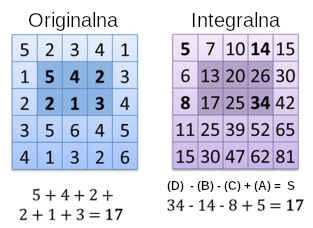
\includegraphics[width=8cm]{integral_image2}
  \caption{Primer računanja površine pravougaonika \cite{IntegralImage1_web}}
  \label{IntegralImage_img2}
\end{figure}

Na slici (\ref{IntegralImage_img2}) je prikazano računanje površine pravougaonika na
originalnoj slici i na integralnoj slici.
Kao što se može videti za površinu pravougaonika MxN na originalnoj slici nam je
potrebno MxN sabiranja. \\
Dok je kod integralne slike broj operacija 2 sabiranja i 2
oduzimanja i ne zavisi od dimenzija pravougaonika.

\begin{equation}
  \Scale[1.4]{\sum\limits_{(x,y)\in ABCD} i(x,y)=ii(D)+ii(A)-ii(B)-ii(C)}
  \cite{Cen2016StudyOV}
  \label{IntegralImage_eq2}
\end{equation}
\newpage

\section{OpenCV modeli} \label{opencv_model}

OpenCV je biblioteka koja sadrži implementacije velikog broja algoritama za
obradu slike.
OpenCV sadrži alat za AdaBoost treniranje kaskadnog klasifikatora kao i implementaciju
detektora objekata pomoću Viola-Jones algoritma. \\
Pored toga OpenCV sadrži istrenirane i testirane modele klasifikatora\footnote{\url{https://github.com/opencv/opencv/tree/master/data/haarcascades}}.
\cite{OpenCV_docs} \\

\noindent
OpenCV istrenirane modele skladišti u .xml fajlove koji sadrže sledeće
informacije o modelu:

\begin{itemize}
	\item Dimenzija obeležja (\emph{height, width})
	\item Broj etapa (\emph{stageNum})
	\item Maksimalan broj obeležja u etapi (\emph{maxWeakCount})
	\item Informacije o etapama (\emph{stages})
    \begin{itemize}
    \item Broj obeležja u etapi (\emph{maxWeakCount})
    \item Prag etape (\emph{stageThreshold})
    \item Informacije o obeležjima (\emph{weakClassifiers})
      \begin{itemize}
      \item Prag obeležja (\emph{internalNodes})
      \item Vrednosti listova (\emph{leafValues})
      \end{itemize}
    \end{itemize}
	\item Informacije o obeležjima (\emph{features})
    \begin{itemize}
    \item Koordinate i težine tačaka pravougaonika (\emph{rects}). \\
      Svako obeležje može imati 2 ili 3 pravougaonika. \\
      Prve 2 vrednosti liste rects su x i y koordinate gornje leve tačke, \\
      treća i četvrta vrednost širina i visina pravougaonika,  \\
      poslednja vrednost je težina pravougaonika.
    \end{itemize}
\end{itemize}

\subsection{OpenCV model za frontalna lica} \label{haarcascade_frontal_sec}

Često korišćeni model za detekciju lica je
\texttt{\detokenize{haarcascade_frontalface_default.xml}}\footnote{\url{https://github.com/opencv/opencv/blob/master/data/haarcascades/haarcascade_frontalface_default.xml}}. \\
Ovaj model se koristi za frontalnu detekciju lica. \\
Neke njegove karakteristike su:
\begin{itemize}
\item Dimenzija obeležja: 24x24
\item Broj etapa: 25
\item Maksimalan broj obeležja u etapi: 211
\item Ukupan broj obeležja: 2913
\end{itemize}

\noindent
Rezultati detekcije ovog modela mogu se videti na
slikama(\ref{sixfaces_scaled},\ref{overexposed_light},\ref{underexposed_light},\ref{rotation_variance},\ref{rotated_res})
iz sekcije \ref{viola_jones_introduction}.
\newpage

\part{Hardverska implementacija}
\section{Sažetak}

Ovaj projekat sadrži:
\begin{itemize}
  \item Projektovanje arhitekture hardverskog akceleratora za Viola-Jones algoritam opisam u delu \ref{viola_jones_algorithm}.
  \item Pisanje specifikacije u Python i C programskom jeziku za izvršavanje i
    pomoć pri particionisanju i projektovanju hardvera.
  \item Pisanje HDL modela za sintezu u SystemVerilog RTL metodologiji i
    \PyGears{} metodologiji.
  \item Pisanje verifikacionog okruženja u SystemVerilog \UVM{} i Python PyGears
    okruženju.
  \item Poređenje dve metodologije i analiza prednosti i mane obe metodologije.
  \item Poređenje komercijalnog \QuestaSim{} simulatora i besplatnog open-source
    \Verilator{} simulatora.
  \item Implementacija projektovanog IP jezgra na \ZTurn{} sa Zynq
    7020 SoC.
  \item Pisanje Linux Kernel drajvera i korisničke aplikacije za korišćenje
    jezgra za detekciju lica na Xilinx Zynq platformi.

\end{itemize}
\newpage
\section{Specifikacije za izršavanje}

Prilikom projektovanja hardverske arhitekture određenog algoritma preporučljivo
je prvo implementirati algoritam u softveru kako bi se algoritam bolje shvatio. \\
Postoje metodologije koje definišu potrebne korake prilikom projektovanja
digitalnih sistema, jedna takva metodologija je \gls{esl}.
U ovom radu nije korišćena ova metodologija već je softverska
specifikacija napisana u C++ i Python jeziku. \\
Iz ovih specifikacija dobijeno je bolje razumevanje algoritma i naznake o
mogućnosti paralelizna određenih delova algoritma i particionisanja komponenti
sistema. \\

\begin{figure}[H]
  \centering
  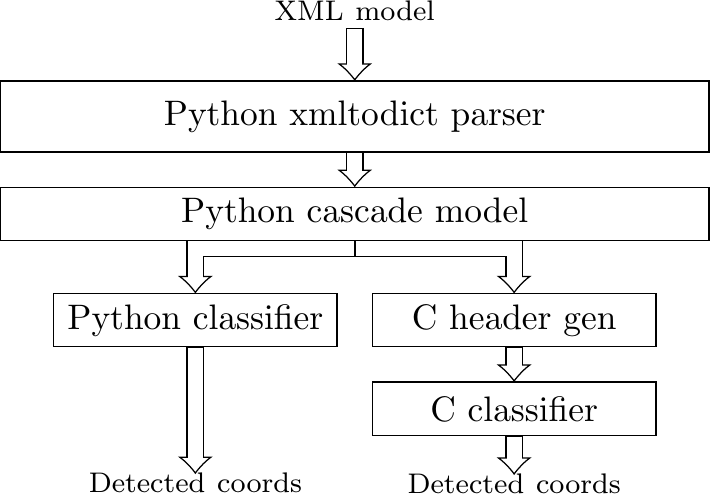
\includegraphics[width=0.9\linewidth]{bdp/sw_arch/sw_arch1.png}
  \caption{Veza Python modela sa XML modelom i C specifikacijom}
  \label{sw_arch_spec1}
\end{figure}

Na slici(\ref{sw_arch_spec1}) prikazana je struktura modela u slučaju Python i C
klasifikatora. \\

\noindent
Na ulazu se nalazi \gls{xml} model dobijen treniranjem pomoću OpenCV biblioteke opisan u sekciji
\ref{opencv_model}. \\
Parsiranje XML modela se rešava u Python-u.
Zbog velikog broja Python paketa dostupnih sa gotovim rešenjima za većinu softverskih problema, problem
parsiranja XML fajla se može rešiti korišćenjem paketa xmltodict\footnote{\url{https://pypi.org/project/xmltodict/}}. \\
\emph{Xmltodict} parsira XML fajl i skladišti ga u Python dictionary. \\
Implementirane su klase \emph{CascadeClass}, \emph{StageClass}, \emph{FeatureClass} i
\emph{RectClass}
\footnote{\texttt{\detokenize{cascade_classifier/python_model/cascade.py}}} koje
predstavljaju abstraktni Python model modela kaskadnog klasifikatora. \\

Napisana je i Python implementacija Viola-Jones algoritma koja koristi Python
model klasifikatora i koristi se kao specifikacija za izvršavanje. \\

Python model klasifikatora može da generiše \emph{C++} reprezentaciju modela
klasifikatora i sačuva ih u Header fajlove. \\
Ovim je izbegnuto parsiranje XML fajlova C++ jezikom, pošto je ovaj zadatak
mnogo jednostavnije odraditi u Python-u. \\
C++ implementacija Viola-Jones algoritma koristi ovako generisan model
klasifikatora.
\newpage
\pgfdeclarelayer{background}
\pgfdeclarelayer{foreground}
\pgfsetlayers{background,main,foreground}

\tikzstyle{cloud1} = [draw=black, thick, fill=red!20, minimum hegiht = 1em]
\tikzstyle{block_l} =[draw, text centered, fill=blue!15, minimum width=3cm, minimum height=3.5cm]
\tikzstyle{block_m} =[draw, text centered, fill=blue!15, minimum width=2.5cm, minimum height=2cm]
\tikzstyle{block_s} =[draw, text centered, fill=blue!15, minimum width=2cm, minimum height=1.5cm]
\tikzstyle{line} = [draw, decoration={markings,mark=at position 1 with {\arrow[scale=2.2,black]{>}}},
    postaction={decorate},
    shorten >=0.4pt]

\begin{tikzpicture}[thick]
  \node [block_l] (img_ram) {IMG RAM};
  \node [coordinate, above = 0cm of img_ram, yshift=-0.5cm, xshift=1.5cm] (img_ram_addr_in){};
  \node [coordinate, left =2.0cm of img_ram] (img_in){};
  \node [coordinate, left = 0cm of img_ram] (img_ram_img_in){};
  \node [coordinate, right = 0cm of img_ram] (img_ram_img_out){};

  \node [block_m, above right = +1cm and 0.2cm of img_ram] (rd_addrgen) {rd\_addrgen};
  \node [coordinate, below = 0cm of rd_addrgen] (rd_addr_addr_out){};

  \node [block_m, above right = -1.75cm and 2.5cm of img_ram ] (ii_gen) {ii\_gen};
  \node [coordinate, left = 0cm of ii_gen] (ii_gen_in){};
  \node [coordinate, right = 0cm of ii_gen] (ii_gen_out){};
  \node [block_m, below = 0.25cm of ii_gen ] (sii_gen) {sii\_gen};
  \node [coordinate, left = 0cm of sii_gen] (sii_gen_in){};
  \node [coordinate, right = 0cm of sii_gen] (sii_gen_out){};

  \node [block_s, right = 1.25cm of sii_gen ] (stddev) {stddev};
  \node [coordinate, above left = -0.25cm and 0cm of stddev] (stddev_ii){};
  \node [coordinate, above left = -0.75cm and 0cm of stddev] (stddev_sii){};
  \node [coordinate, right = 0cm of stddev] (stddev_out){};

  \node [block_m, right = 1.0cm of ii_gen ] (frame_buffer) {frame\_buffer};
  \node [coordinate, left = 0cm of frame_buffer] (frame_buffer_in){};
  \node [coordinate, above left = -0.5cm and 0cm of frame_buffer] (frame_buffer_rect_addr){};
  \node [coordinate, right = 0cm of frame_buffer] (frame_buffer_out){};

  \node [block_m, above = 1.0cm of frame_buffer ] (features_mem) {features\_mem};
  \node [coordinate, left = 0cm of features_mem] (rects_addr){};
  \node [coordinate, right = 0cm of features_mem] (rects_weights){};

  \node [block_l, fill=red!15, above right = -3.5cm and 1cm of frame_buffer] (classifier) {\huge Classifier};
  \node [coordinate, above left = -1cm and 0cm of classifier] (classifier_ii){};
  \node [coordinate, above left = -2.5cm and 0cm of classifier] (classifier_stddev){};
  \node [coordinate, above left = -0.5cm and 0cm of classifier] (classifier_weights){};
  \node [coordinate, above right = -1.0cm and 0cm of classifier] (detected_addr){};
  \node [coordinate, above right = -2.5cm and 0cm of classifier] (irq){};

  %% group %%
 \begin{pgfonlayer}{background}
  \node[inner sep=7pt, fill=yellow!25, rounded corners, inner ysep =30pt, draw, thick,fit=(img_ram) (rd_addrgen) (ii_gen) (features_mem) (sii_gen) (frame_buffer) (stddev) (classifier)] (ip_core) {};
  \node[above left] at (ip_core.south east) {\huge Cascade Classifier IP core};
\end{pgfonlayer}

  % arrows
  \path [line] (rd_addr_addr_out)  |- (img_ram_addr_in) node[transition, xshift=0.8cm, yshift=0.25cm] {rd\_addr};
  \path [line] (img_in) node[transition, yshift=0.25cm, xshift=0.65cm]{\large img\_in} -- (img_ram_img_in);
  \path [line] (img_ram_img_out) node[transition, yshift=0.2cm, xshift=0.9cm] {img\_out} -- +(1.75cm, 0cm) |- (ii_gen_in);
  \path [line] (img_ram_img_out) -- +(1.75cm, 0cm) |- (sii_gen_in);
  \path [line] (ii_gen_out) -- +(0.5cm, 0cm) node[transition, yshift=0.2cm, xshift=0cm] {ii} |- (stddev_ii);
  \path [line] (sii_gen_out) -- +(0.5cm, 0cm)  node[transition, yshift=0.2cm, xshift=0cm] {sii} |- (stddev_sii);
  \path [line] (ii_gen_out) |- (frame_buffer);
  \path [line] (frame_buffer_out) node[transition, yshift=+0.2cm, xshift=0.5cm] {fb\_ii} |- (classifier_ii);
  \path [line] (stddev_out) -- +(0.5cm, 0) node[transition, yshift=-0.2cm, xshift=0.1cm] {stddev} |- (classifier_stddev);
  \path [line] (rects_addr) node[transition, yshift=+0.2cm, xshift=-1.1cm] {rects\_addr}  -- +(-0.5cm, 0cm) |- (frame_buffer_rect_addr);
  \path [line] (rects_weights) node[transition, yshift=+0.2cm, xshift=+1.2cm] {rects\_weights}  -- +(+0.5cm, 0cm) |- (classifier_weights);
  \path [line] (detected_addr) -- +(3.0cm, 0cm) node[transition, yshift=0.25cm, xshift=-1.1cm]{\large detect\_addr} ;
  \path [line] (irq) -- +(3.0cm, 0cm) node[transition, yshift=0.25cm, xshift=-0.4cm]{\large irq} ;
\end{tikzpicture}

\newpage
\newpage

\section{PyGears metodologija} \label{pygears_sec}

\subsection{Uvod}

PyGears\cite{pygears_site} pozajmljuje koncepte iz funkcionalnog programiranja i primenjuje ih na
dizajn digitalnog hardvera \\
Sastoji se od Gears metodologije i Python Framework koji implementira Gears metodologiju. \\
Gears metodologija omogućava lako povezivanje i kompozabilnost sistema pomoću manjih
funkcionalnih jedinica pod nazivom gear-ovi. \\
Gear moduli su međusobno povezani \gls{dti} interfejsom koji implementira jednostavan
handshake protokol.
Korišćenjem standardnog generičkog interfejsa omogućeno je lako povezivanje ovih
komponenti. \\

Opisom hardvera u Python-u koji je dinamičan jezik i veoma visokog nivoa mogu se
napisati gear-ovi koji su veoma apstraktni i generički, time je omogućeno lako
ponovno korišćenje modela. \\

PyGears takođe omogućava i verifikaciju u Python-u. Implementiran je interfejs
ka popularnim komercijalnim simulatorima Questa, NCSim i open source Verilator,
tako da je moguća kosimulacija između Python okruženja i \gls{hdl} modela. \\

PyGears konačno obavlja konverziju Python opisa u \gls{sv} opis koji
je podržan od strane alata za sintezi i simulaciju.

\subsection{Poređenje sa RTL metodologijom}

PyGears\cite{PyGears_OSDA} predstavlja alternativu \gls{rtl}\cite{chu2006rtl} metodologiji za opis hardvera.
RTL metodologija pruža standardan način translacije sekvencijalnog algoritma u
hadverski opis.
Struktura dobijena pomoću RTL metodologije uglavnom se sastoji od \textbf{\gls{fsmd}}. \\
Datapath sadrži funkcionalne i memorijske jedinice i mreže za rutiranje podataka\cite{PSDS_5} \\
Controlpath diriguje podacima u Datapath delu i sačinjen je od mašine stanja.\\

Kako dizajn implementiran pomoću RTL metodologije postaje kompleksniji i mašina
stanja postaje kompleksnija i sadrži više stanja.
Pipeline-ovanje, debagovanje  ovakvog dizajna može biti veoma teško. \\
Prednost Gears metodologije u odnosu na RTL metodologiju najvidljivija je u
sistemima koji su Dataflow orijentisani.

\subsection{Jezici za opis hardvera}

Jezici sa opis hardvera koji se danas daleko najviše koriste su Verilog i VHDL,
nastali su 1984. i 1983. godine i daleko su siromašniji po mogućnostima od današnjih
jezika višeg nivoa kao što su Python, C++. \\
Najveća prednost ovih jezika je podrška od strane alata za sintezu i simulaciju,
kako se ovi jezici koriste za opis i verifikaciju hardvera preko 30 godina,
alati su zreli i dobro istestirani. \\

Sve kompanije koje proizvode FPGA čipove trenutno ne objavljuju
arhitekturu svojih FPGA čipova, pa alati za sintezu i implementaciju zavise od
tih kompanija\footnote{Postoji inicijativa da se dokumentuju FPGA čipovi svih velikih
proizvođača u projektu zvanom SymbiFlow\cite{SymbiFlow}.}
.
Zbog toga direktna podrška alata za sintezu i implementaciju za neki novi HDL jezik je
nemoguća. \\

Iz tog razloga većina novih HDL jezika baziranih na
Python\cite{decaluwe2004myhdl, PyGears_OSDA}, Scala
\cite{bachrach2012chisel, SpinalHDL}, Haskell\cite{baaij2010c} generišu konačan
HDL kod u Verilog-u, SystemVerilog-u ili VHDL-u pogodnom za simulatore i alate
za sintezu. \\

Dok se ovi jezici uglavnom baziraju na RTL metodologiji i uvode jezik višeg
nivoa kao zamenu za standardan HDL.
PyGears dodatno izdvaja i uvođenje nove metodologije zvane Gears.

\subsection{Gears metodologija}
Gears metodologija obezbeđuje bolju kompozabilnost i ponovno korišćenje
napisanih hardverskih modela. \\
Kako bi se ovo postiglo uveden je standardan generički handshaking interfejs za
komunikaciju između modula.

\subsubsection{DTI interfejs}
\begin{figure}[H]
  \centering
  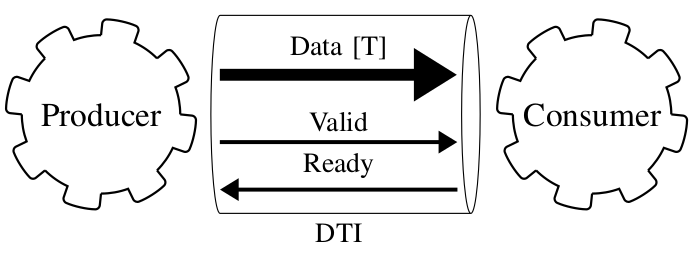
\includegraphics[width=0.5\linewidth]{dti}
  \caption{DTI interfejs\cite{PyGears_OSDA}}
  \label{DTI_intf_img}
\end{figure}

Jednostavan \textbf{\gls{dti}} interfejs se koristi za komunikaciju između gear-ova.
Modul koji šalje podatke se naziva Producer, a modul koji prima podatke se
naziva Consumer. \\
DTI se sastoji od sledećih signala:
\begin{itemize}
\item \textbf{Data} linije za podatke, proizvolje širine i proizvoljnog tipa.
\item \textbf{Valid} jednobitan signal kojim upravlja Producer i signalizira da
  je podataka na Data liniji validan.
\item \textbf{Ready} jednobitan signal kojim upravlja Consumer i signalizira da je
  konzumirao podatak sa Data linije i spreman za novi podatak.
\end{itemize}
Pomoću Valid i Ready signala realizovan je handshaking protokol. \\

\begin{figure}[H]
  \centering{
    \resizebox{0.75\textwidth}{!}{%
      \\
\begin{tikztimingtable}[%
    timing/dslope=0.1,
    timing/.style={x=5ex,y=2ex},
    x=5ex,
    timing/rowdist=4ex,
    timing/name/.style={font=\sffamily\scriptsize}
]
\busref{CLK}         & 18{c} \\
\busref{Data}      & 2u 3D 2U 1D 0L 1D 1U \\
\busref{Valid}   & 1L 3H 2L 2H L \\
\busref{Ready} & 3L 5H L  \\
\busref{Event}     & 3U 1D{ACK} 2U 1D{ACK} 1D{ACK} U\\
\extracode
\begin{pgfonlayer}{background}
\begin{scope}[semitransparent ,semithick]
\vertlines[darkgray,dotted]{0.5,1.5 ,...,8.0}
\foreach \i [count=\col from 0] in {0.5,1.5,...,8.0}
    \node[font=\scriptsize] at (\i,3) {${\col}$};
\end{scope}
\end{pgfonlayer}
\end{tikztimingtable}

    }}
  \caption{DTI primer transakcije}
  \label{dti_example1}
\end{figure}

Na slici(\ref{dti_example1}) prikazan je talasni oblik protokola:
\begin{enumerate}
\item Producer je postavio podatak na Data liniju i podigao Valid signal na
  jedinicu. Što označava validan podatak na magistrali.
\item Istog trenutka nakon postavljanja Valid signala na jedinicu Consumer može
  da koristi podatak na magistrali.
\item Consumer može koristiti podatak potreban broj taktova.
\item Kada Consumer završi sa korišćenjem podatka, postavlja Ready signal na
  jedinicu čime označava ACK(acknowledgment) odnosno signalizira da je završio
  sa podatkom na magistrali i da je spreman za sledeći podatak. \\
  Nakon handshake-a Producer može postaviti novi podatak na magistralu.
\item Producer ne sme menjati podatak na magistrali sve do pojave ACK od strane
  Consumera.
\item Producer može držati Valid signal na logičkoj nuli i tada se neće
  obavljati transakcije na magistrali.
\item Ne sme postojati kombinaciona putanja od Ready do Valid signala na strani
  Producer-a.
  Odnosno Producer ne sme odlučivati o postavljanju podatka na magistrali na
  osnovu stanja Consumer-a.
\item Može postojati kombinaciona putanja od Valid do Ready signala na strani
  Consumer-a.

\end{enumerate}

\subsection{Tipovi podataka} \label{pygears_data_types}

Data linija u DTI interfejsu pored toga što može biti proizvoljne širine može
predstavljati i različite kompleksne tipove podataka.
Ovim se omogućava bolja kompozicija modula, lakša manipulacija podacima,
pregledniji izvorni kod.

\subsubsection{Uint} \label{uint_sec}
\textbf{Uint[W]} predstavlja neoznačenu celobrojnu vrednost proizvoljne
širine W.

\subsubsection{Int} \label{int_sec}
\textbf{Int[W]} predstavlja označenu celobrojnu vrednost proizvoljne
  širine W.

\subsubsection{Tuple} \label{tuple_sec}
\textbf{Tuple[T1, T2, ..., TN]} predstavlja tip sličan strukturi gde
  polja Tn mogu biti bilo kog tipa. \\
  Koordinate piksela slike mogu se prigodno predstaviti kao Tuple tip. \\
  Na primer Tuple[Uint[W\_Y], Uint[W\_X]] ovaj Tuple sadrži dva Uint polja koji
  predstavljaju X i Y koordinate.

\subsubsection{Array} \label{array_sec}
\textbf{Array[T, N]} predstavlja niz od N podataka tipa T.

\subsubsection{Float}
\textbf{Float} se koristi za predstavljanje decimalnih brojeva pomoću formata
sa pokretnom tačkom.
Ovaj tip se koristi isključivo za simulaciju i ne može se implementirati u hardveru.

\subsubsection{Fixp}
\textbf{Fixp[WI, W]} se koristi za predstavljanje decimalnih brojeva sa fiksnom tačkom. \\
Format Fixed point tipa je \textbf{WI} širina celobrojnog dela i \textbf{W}
ukupna širina magistrale, širina decimalnog dela je razlika ove dve širine. \\
Ovaj tip se koristi za reprezentaciju decimalnih brojeva u hardveru.

\subsubsection{Queue} \label{queue_sec}
\textbf{Queue[T, LVL]} ili red predstavlja transakciju koja sadrži više
podataka proizvoljnog tipa T i informaciju o završetku transakcije EOT(end of
transaction).
Queue može biti proizvoljnog nivoa LVL. \\
Kao primer \textbf{Queue[Uint[4], 1](0, 1, 2, 3)} predstavlja red od četiri
četvorobitna podatka, primer talasnih oblika na slici ispod.
Rezultujuća Data magistrala biće širine 5 bita, 4 bita za podatak i 1 bit za EOT.

\begin{figure}[H]
  \centering{
    \resizebox{0.6\textwidth}{!}{%
      \\
\begin{tikztimingtable}[%
    timing/dslope=0.1,
    timing/.style={x=5ex,y=2ex},
    x=5ex,
    timing/rowdist=4ex,
    timing/name/.style={font=\sffamily\scriptsize}
]
\busref{CLK}         & 12{c} \\
\busref{Data}[4:0]      & 2u 1D{0x00} 1D{0x01} 1D{0x02} 1 D{0x13}  U \\
\busref{Data[3:0]} & 2u 1D{0} 1D{1} 1D{2} 1D{3} U \\
\busref{EOT\textsubscript{(Data[4])}} & U 3L 1H U \\
\busref{Valid}   & 1L 4H L \\
\busref{Ready} & 4L 1H L  \\
\busref{Event}     & 4U 1D{ACK} U \\
\extracode
\begin{pgfonlayer}{background}
\begin{scope}[semitransparent ,semithick]
\vertlines[darkgray,dotted]{0.5,1.5 ,...,6.0}
\foreach \i [count=\col from 0] in {0.5,1.5,...,6.0}
    \node[font=\scriptsize] at (\i,3) {${\col}$};
\end{scope}
\end{pgfonlayer}
\end{tikztimingtable}
    }}
  \caption{Primer transakcije tipa}
  \label{queue_img1}
\end{figure}

Dvodimenzionalna matrica se može predstaviti kao Queue[Uint[4], 2],
odnosno red nivoa 2 sa proizvoljnim podatkom u ovom slučajem četvorobitnim
neoznačnim brojem.

\begin{figure}[H]
  \centering{
    \resizebox{0.25\textwidth}{!}{%
      \begin{tikzpicture}
  % draw the grid and the numbers
  \draw (-1,-1) grid (2,2) foreach \i in {0,...,2}{
    (\i-.5,2.5) node{\i} (-1.5,1.5-\i) node{\i}};

  \node[text width=1.5cm] at (0.0,1.5) (A_coord) {\large \textbf{5}};
  \node[text width=1.5cm] at (1.0,1.5) (A_coord) {\large \textbf{1}};
  \node[text width=1.5cm] at (2.0,1.5) (A_coord) {\large \textbf{9}};

  \node[text width=1.5cm] at (0.0,0.5) (A_coord) {\large \textbf{3}};
  \node[text width=1.5cm] at (1.0,0.5) (A_coord) {\large \textbf{7}};
  \node[text width=1.5cm] at (2.0,0.5) (A_coord) {\large \textbf{11}};

  \node[text width=1.5cm] at (0.0,-0.5) (A_coord) {\large \textbf{0}};
  \node[text width=1.5cm] at (1.0,-0.5) (A_coord) {\large \textbf{4}};
  \node[text width=1.5cm] at (2.0,-0.5) (A_coord) {\large \textbf{15}};

\end{tikzpicture}

    }}
\caption{Matrica veličine 3x3}
\label{queue_matrix1}
\end{figure}

\begin{figure}[H]
\centering{
  \resizebox{.9\textwidth}{!}{%
    \\
\begin{tikztimingtable}[%
    timing/dslope=0.1,
    timing/.style={x=5ex,y=2ex},
    x=5ex,
    timing/rowdist=4ex,
    timing/name/.style={font=\sffamily\scriptsize}
]
\busref{CLK}         & 22{c} \\
\busref{Data}[5:0]      & 2u 1D{0x05} 1D{0x01} 1D{0x19} 1D{0x03} 1D{0x07}
1D{0x1B} 1D{0x00} 1D{0x04} 1D{0x1F} U \\
\busref{Data[3:0]} & 2u 1D{5} 1D{1} 1D{9} 1D{3} 1D{7} 1D{11} 1D{0} 1D{4} 1D{15}  U \\
\busref{EOT[1]\textsubscript{(Data[5])}} & U 6L 3H U \\
\busref{EOT[0]\textsubscript{(Data[4])}} & U 2L 1H 2L 1H 2L 1H U \\
\busref{Valid}   & 1L 9H L \\
\busref{Ready} & 9L 1H L  \\
\busref{Event}     & 9U 1D{ACK} U \\
\extracode
\begin{pgfonlayer}{background}
\begin{scope}[semitransparent ,semithick]
\vertlines[darkgray,dotted]{0.5,1.5 ,...,11.0}
\foreach \i [count=\col from 0] in {0.5,1.5,...,11.0}
    \node[font=\scriptsize] at (\i,3) {${\col}$};
\end{scope}
\end{pgfonlayer}
\end{tikztimingtable}

  }}
\caption{Transakcija matrice \ref{queue_matrix1}}
\label{queue_matrix2}
\end{figure}

Kao što se može videti linija za podatke je u ovom slučaju širine 6 bita, od
toga 2 bita su EOT. \\
Na slici(\ref{queue_matrix1}) u taktovima(3, 6, 9) niži bit EOT-a je na visokom nivou
što predstavlja podatak u poslednjoj koloni matrice.
U taktovima(7, 8, 9) viši bit EOT-a je na visokom nivou što označava podatke u poslednjoj
liniji matrice.
Konačno u taktu 9 oba EOT bita su na visokom nivou što označava poslednji podatak u matrici.

\subsubsection{Union} \label{union_sec}
\textbf{Union[T1, T2, ..., TN]} je unija koja može prenositi samo jedan od
  podataka Tn u trenutku.
  Uz podatak prenosi se i informacija o aktivnom podatku na magistrali.

\subsubsection{Unit} \label{unit_sec}
\textbf{Unit} je tip koji prenosi ``prazan'' podatak.

\begin{figure}[H]
\centering{
  \resizebox{.35\textwidth}{!}{%
    \\
\begin{tikztimingtable}[%
    timing/dslope=0.1,
    timing/.style={x=5ex,y=2ex},
    x=5ex,
    timing/rowdist=4ex,
    timing/name/.style={font=\sffamily\scriptsize}
]
\busref{CLK}         & 6{c} \\
\busref{Valid}   & 1L 1H L \\
\busref{Ready} & 1L 1H L  \\
\busref{Event}     & 1U 1D{ACK} U \\
\extracode
\begin{pgfonlayer}{background}
\begin{scope}[semitransparent ,semithick]
\vertlines[darkgray,dotted]{0.5,1.5 ,...,3.0}
\foreach \i [count=\col from 0] in {0.5,1.5,...,3.0}
    \node[font=\scriptsize] at (\i,3) {${\col}$};
\end{scope}
\end{pgfonlayer}
\end{tikztimingtable}
  }}
\caption{Unit tip}
\label{unit_img1}
\end{figure}

\subsection{Čistoća Gear-ova} \label{gear_purity}

Kako bi se gear-ovi lakše povezivali i njihova funkcionalnost i ponašanje bilo
razumljivo i predvidljivo dizajneru, preporučuje se pisanje ``čistih''  gear-ova. \\
``Čist'' gear je onaj čije je inicijalno stanje dobro poznato i koji će se nakon
izvršene funkcionalnosti potpuno vratiti u inicijalno stanje. \\
Čisto kombinacioni gear-ovi su uvek ``čisti''.

\newpage
\subsection{Definicija Gear komponenti}

PyGears trenutno podržava tri načina za implementaciju Gear komponenti.

\begin{code}[H]{python}{Primer definisanja Gear komponente}{gear_example1}
@gear
def gear_name(in1: T1, ..., inN: TN,
              *,
              p1=dflt, ..., pM=dfltM) -> ReturnType:
    # Gear implementation
\end{code}

Primer(\ref{gear_example1}) prikazuje definisanje gear komponente. \\
Dekorator \textbf{@gear} označava da je funkcija gear\_name zapravo Gear komponenta,
slično kao module ili entity kod Verilog-a i VHDL-a. \\
Kao parametri funkcije prosleđuju se DTI interfejsi i generički parametri.
Delimiter ``*'' označava početak generičkih parametara. \\

Ulazni DTI interfejsi mogu imati proizvoljan naziv i tipove opisane u
sekciji(\ref{pygears_data_types}). \\
Parametar može biti bilo koji Python objekat i može imati inicijalnu vrednost dflt.

\subsubsection{Gear implementiran pomoću SystemVerilog-a}

Jedan od mogućih načina implementacije Gear komponente je pisanje SystemVerilog
opisa pa zatim Python wrapper-a za komponentu. \\
Prilikom pisanja modula na ovaj način potrebno je pobrinuti se da napisana
komponenta poštuje DTI protokol kao i da je ``čist'' Gear(\ref{gear_purity}). \\

Prilikom pisanja wrapper-a za ovako implementiranu komponentu potrebno je
unapred odrediti ReturnType koji će odgovarati izlaznom interfejsu SystemVerilog modula. \\
Takođe deo za implementaciju Gear-a u Python-u može ostati prazan. \\

Kako postoji velika verovatnoća unošenja bagova u dizajn prilikom ručnog pisanja
modula koji poštuje DTI interfejs i koji je ``čist'', ovaj način implementacije
modula nije preporučen.

\subsubsection{Gear implementiram kompozicijom}

Kako PyGears dolazi sa bibliotekom osnovnih funkcionalnih modula, većina
potrebnih funkcionalnosti moguće je ostvariti njihovom kompozicijom. \\

\newpage

\subsubsection{Gear implementiram Python to HDL kompajlerom}

Moguće je i pisati opis gear-a u Python-u pomoću HDL kompajlera. \\

Kao primer prikazan je serialize gear koji kao ulaz prima niz podataka, a na
izlazu daje jedan po jedan podatak ulaznog niza, odnosno serializuje podatke.

\begin{code}[H]{python}{Primer kompajliranog serialize gear-a}{serialize_example}
@gear(svgen={'compile': True})
async def serialize(din: Array) -> b'din.dtype':
    async with din as val:
        for i in range(len(din.dtype)):
            yield val[i]
\end{code}

Kao primer možemo uzeti niz \textbf{Array[Uint[4], 3](3, 7, 9)} za očekivati je da će se
na izlazu pojaviti podaci redom 3, 7 pa 9 što je prikazano na slici \ref{serialize_example2}.
\begin{figure}[H]
\centering{
  \resizebox{.55\textwidth}{!}{%
    \\
\begin{tikztimingtable}[%
    timing/dslope=0.1,
    timing/.style={x=5ex,y=2ex},
    x=5ex,
    timing/rowdist=3ex,
    timing/name/.style={font=\sffamily\scriptsize}
]
\busref{CLK}         & 10{c} \\
\busref{din}      & 1U 3D{0x973} U \\
\busref{din[2]}      & 1U 3D{0x9} U \\
\busref{din[1]}      & 1U 3D{0x7} U \\
\busref{din[0]}      & 1U 3D{0x3} U \\
\busref{din\_valid}   & 1L 3H L \\
\busref{din\_ready} & 3L 1H L  \\
\busref{dout}      & 1U 1D{0x3} 1D{0x7} 1D{0x9} U \\
\busref{dout\_valid}   & 1L 3H L \\
\busref{dout\_ready} & 1L 3H L  \\
\extracode
\begin{pgfonlayer}{background}
\begin{scope}[semitransparent ,semithick]
\vertlines[darkgray,dotted]{0.5,1.5 ,...,4.0}
\foreach \i [count=\col from 0] in {0.5,1.5,...,4.0}
    \node[font=\scriptsize] at (\i,3) {${\col}$};
\end{scope}
\end{pgfonlayer}
\end{tikztimingtable}

  }}
\caption{Serialize gear primer}
\label{serialize_example2}
\end{figure}

\newpage

\bibliography{bibliography}
\bibliographystyle{IEEEtran}

\end{document}